\documentclass{mcmthesis}
  \makeatletter
  \newcommand{\rmnum}[1]{\romannumeral #1}
  \newcommand{\Rmnum}[1]{\expandafter\@slowromancap\romannumeral #1@}
  \makeatother

\mcmsetup{CTeX = false,   % 使用 CTeX 套装时,设置为 true
        tcn = 91397, problem = C,
        sheet = true, titleinsheet = true, keywordsinsheet = true,
        titlepage = false, abstract = true}
\usepackage{palatino}
\usepackage{lipsum}
\usepackage{cite}
\usepackage{amsmath}  
\usepackage{amssymb}
\usepackage{url}
\usepackage{subfigure}
\usepackage{indentfirst} 
\usepackage{float}

\setlength{\parindent}{1.5em}
\title{}
\begin{document}
\begin{abstract}
abstract
\begin{keywords}
keyword1; keyword2
\end{keywords}
\end{abstract}
\maketitle


\tableofcontents
% \thispagestyle{}% 当前页不显示页码'
\pagestyle{fancy} 
\rhead{\small\sffamily  \rmnum{\thepage}}
\newpage
\pagestyle{fancy}
\rhead{\small\sffamily Page \thepage\ of \pageref{LastPage}}
\setcounter{page}{1}

\section{Introduction}
\subsection{Statement of the problem}
Energy production and energy consumption, which can be regarded as an important economic index, not only reflect the industrial development of a country but also relate to the lifehood of a country. But on the other hand, with the continuous advancement and deepening of the industrialization of human civilization, the consumption of non-renewable energy sources such as coal, petroleum is also accelerating. Hence, the development of cleaner renewable energy is particularly important. After all, if humans depend too much on non-renewable energy sources, the day when fossil fuels are depleted is also a day for humankind to return to agrarian society.

As the world's superpower, the US is a big country of energy. Many of America's energy policy decentralizes to the state level. to ensure cooperative action between the states\cite{InterstateCompact}, many compacts are formed between states. In this context, along the border with Mexico four states, California, Arizona, new Mexico, Texas hope to form a new energy compact focused on more and more widely used, cleaner renewable energy sources.
\begin{itemize}
  \item Create an energy profile for each of the four states.
  \item Make governors easier to understand the four states'usage of cleaner, renewable energy sources  and the similarities and difference between the four states.
  \item Determine a state that is appeared to have the ``best" profile for use of cleaner, renewable energy in 2009.
  \item Predict the energy profile of each state in 2025 and 2050.
  \item Determine renewable energy usage targets for 2025 and 2050 which are also for the new four-state energy compact.
  \item Provide at least three suggestions about how to meet the energy compact goals.
\end{itemize}

\subsection{Overview of Our Work}
\begin{itemize}
  \item 
\end{itemize}

\section{Notations and Assumptions}
\subsection{Notations}
\begin{table}[H]
  \centering
  \begin{tabular}{ll}
    \toprule
    Symbol & Specification \\
    \toprule
    $T_s$  &  The total energy transferred. \\
    $T_e$  &  The renewable energy transferred.\\
    $S_p$  &  The total energy produced.\\
    $E_p$  &  The renewable energy producted.\\
    $S_c$  &  The total energe consumed.\\
    $E_c$  &  The renewable energy consumed.\\
    $C_i$  &  The proximity of the i-th evaluation object with the optimal solution.\\
    $D^-_i$  &  The distance between the i-th evaluation object and the worst case.\\
    $D^+_i$  &  The distance between the i-th evaluation object and the best case.\\
    $E^*$  &  The energy status indicator.\\
    $E$    &  The impact of energy, economy or environment.\\
    $W_{si}$  &  The subjective evaluation weight of indicator I.\\
    $W_{oi}$  &  The objective evaluation weight of indicator I.\\
    $W_{ti}$  &  The overall weight of indicator I.\\    

    \bottomrule
  \end{tabular}
\end{table}

\subsection{Assumptions}

\section{Energy Profile}
\subsection{Overview}
We make an energy profile for the four states from 1960 to 2009 in the past 50 years, which covers four aspects of energy consumption, energy prices, energy expenditures, energy production.As shown in the following figures.

(Note that the following figures labels are five-character series names.The first two letters  represent state code. According to the guide \cite{pr_guide}, \cite{use_guide}, \cite{product}, the third and fourth letters like 'TC' means total consumption and 'PR' means product; the fifth letter represents the type of data such as 'B' means consumption in British thermal units (Btu), 'D' means price in dollars per million Btu and 'V' means expenditure in million dollars.Furthemore, the curve represents the change in energy over time.) 

\subsection{Each State}
\subsubsection{Arizona}
\begin{figure}[H]
\begin{minipage}[htb]{0.5\textwidth}
\centering
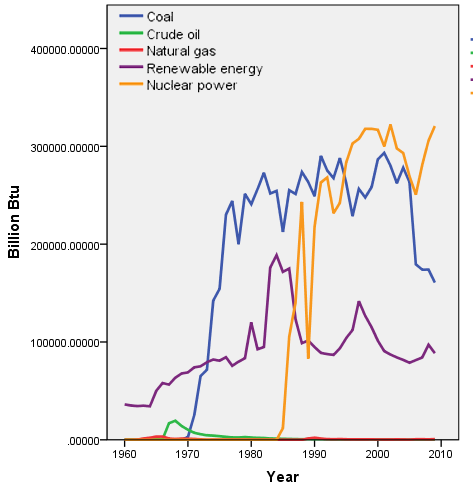
\includegraphics[width=3in]{AZPRB.png}
\caption{AZPRB} \label{fig:AZPRB}
\end{minipage}
\begin{minipage}[htb]{0.5\textwidth}
\centering
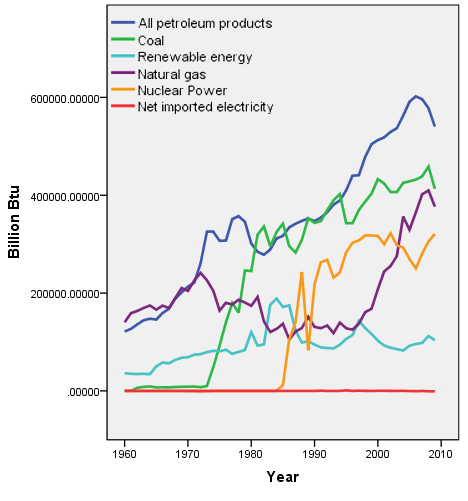
\includegraphics[width=3in]{AZTCB.png}
\caption{AZTCB} \label{fig:AZTCB}
\end{minipage}
\end{figure}

\begin{figure}[H]
\begin{minipage}[htb]{0.5\textwidth}
\centering
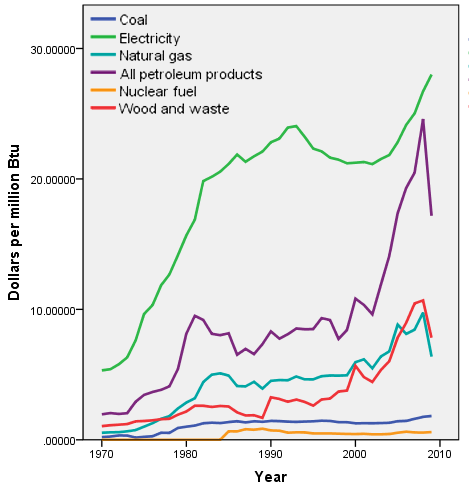
\includegraphics[width=3in]{AZTCD.png}
\caption{AZTCD} \label{fig:AZTCD}
\end{minipage}
\begin{minipage}[htb]{0.5\textwidth}
\centering
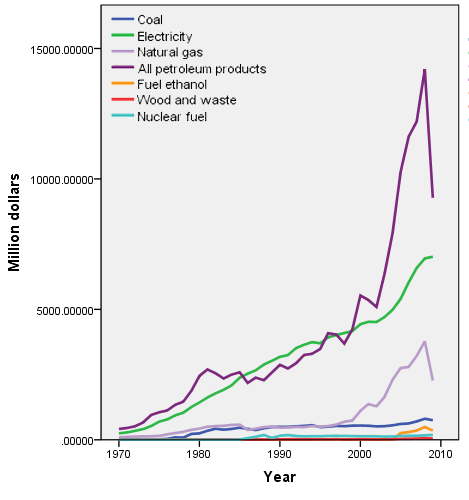
\includegraphics[width=3in]{AZTCV.png}
\caption{AZTCV} \label{fig:AZTCV}
\end{minipage}
\end{figure}


\subsubsection{California}
\begin{figure}[H]
\begin{minipage}[htb]{0.5\textwidth}
\centering
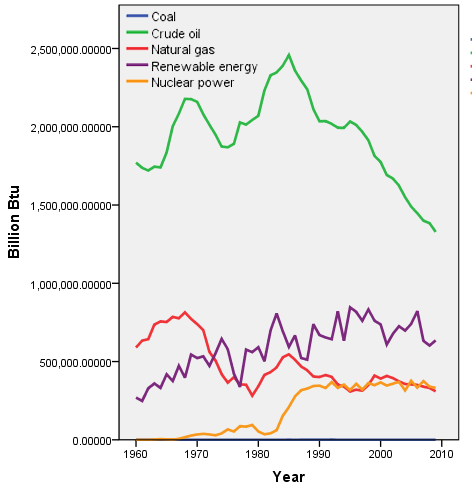
\includegraphics[width=3in]{CAPRB.png}
\caption{CAPRB} \label{fig:CAPRB}
\end{minipage}
\begin{minipage}[htb]{0.5\textwidth}
\centering
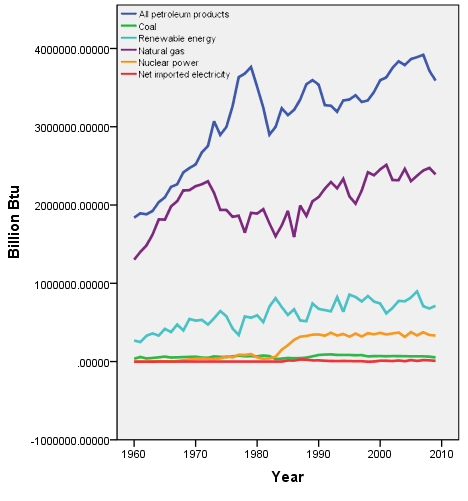
\includegraphics[width=3in]{CATCB.png}
\caption{CATCB} \label{fig:CATCB}
\end{minipage}
\end{figure}

\begin{figure}[H]
\begin{minipage}[htb]{0.5\textwidth}
\centering
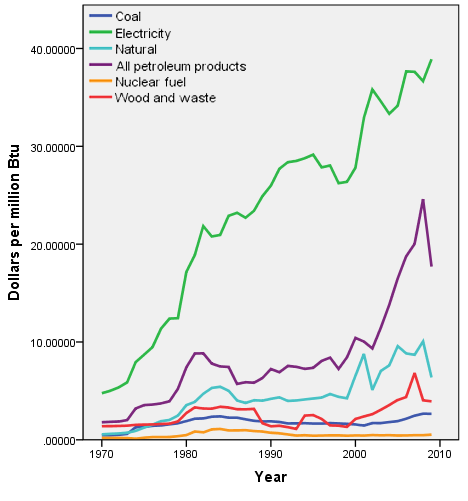
\includegraphics[width=3in]{CATCD.png}
\caption{CATCD} \label{fig:CATCD}
\end{minipage}
\begin{minipage}[htb]{0.5\textwidth}
\centering
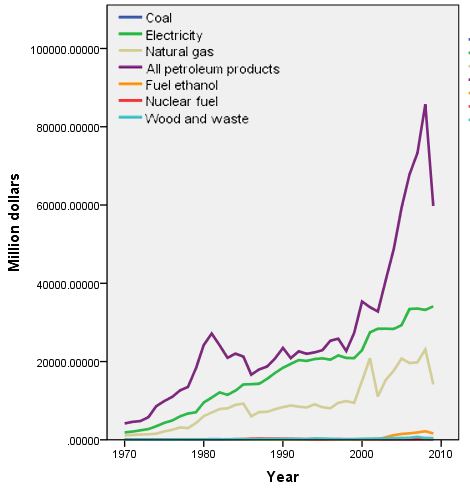
\includegraphics[width=3in]{CATCV.png}
\caption{CATCV} \label{fig:CATCV}
\end{minipage}
\end{figure}

\subsubsection{New Mexico}
\begin{figure}[H]
\begin{minipage}[htb]{0.5\textwidth}
\centering
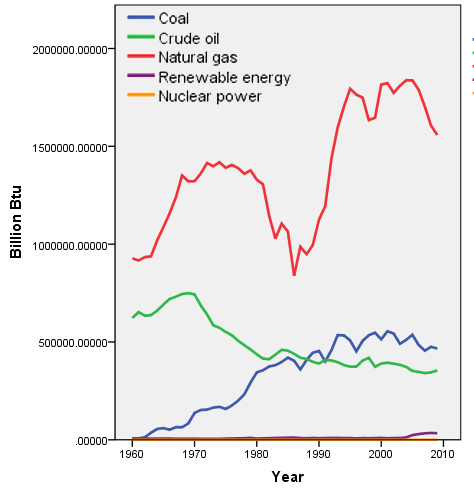
\includegraphics[width=3in]{NMPRB.png}
\caption{NMPRB} \label{fig:NMPRB}
\end{minipage}
\begin{minipage}[htb]{0.5\textwidth}
\centering
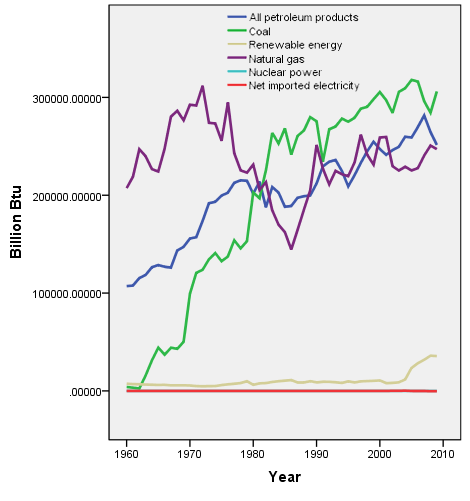
\includegraphics[width=3in]{NMTCB.png}
\caption{NMTCB} \label{fig:NMTCB}
\end{minipage}
\end{figure}

\begin{figure}[H]
\begin{minipage}[htb]{0.5\textwidth}
\centering
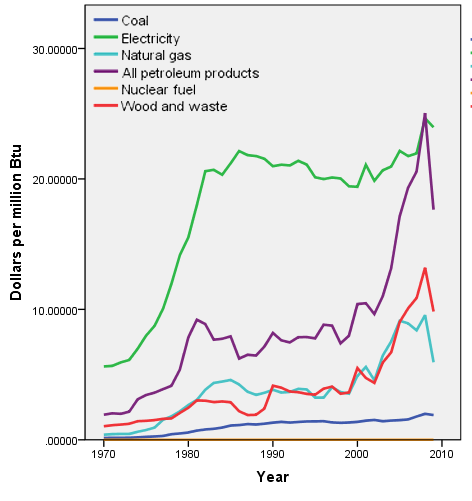
\includegraphics[width=3.in]{NMTCD.png}
\caption{NMTCD} \label{fig:NMTCD}
\end{minipage}
\begin{minipage}[htb]{0.5\textwidth}
\centering
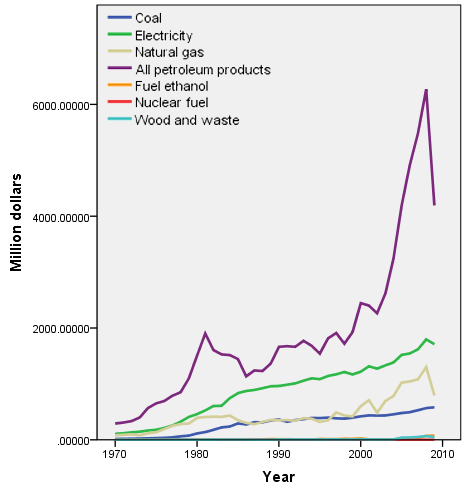
\includegraphics[width=3in]{NMTCV.png}
\caption{NMTCV} \label{fig:NMTCV}
\end{minipage}
\end{figure}

\subsubsection{Texas}
\begin{figure}[H]
\begin{minipage}[htb]{0.5\textwidth}
\centering
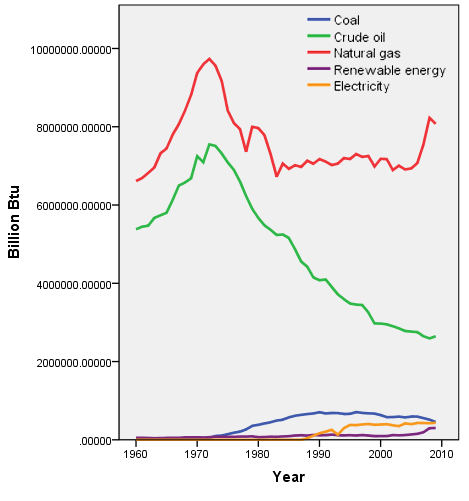
\includegraphics[width=3in]{TXPRB.png}
\caption{TXPRB} \label{fig:TXPRB}
\end{minipage}
\begin{minipage}[htb]{0.5\textwidth}
\centering
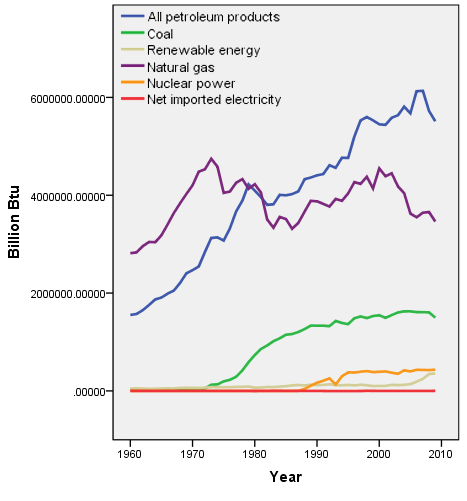
\includegraphics[width=3in]{TXTCB.png}
\caption{TXTCB} \label{fig:TXTCB}
\end{minipage}
\end{figure}

\begin{figure}[H]
\begin{minipage}[htb]{0.5\textwidth}
\centering
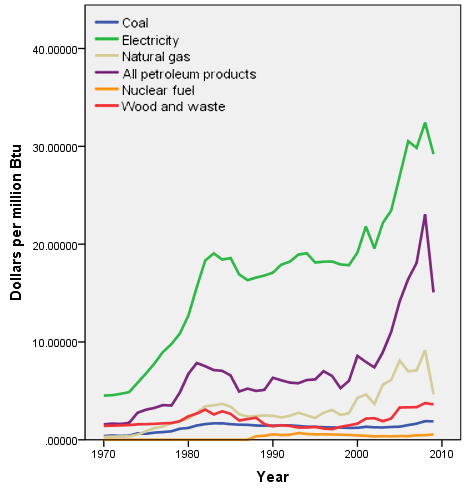
\includegraphics[width=3in]{TXTCD.png}
\caption{TXTCD} \label{fig:TXTCD}
\end{minipage}
\begin{minipage}[htb]{0.5\textwidth}
\centering
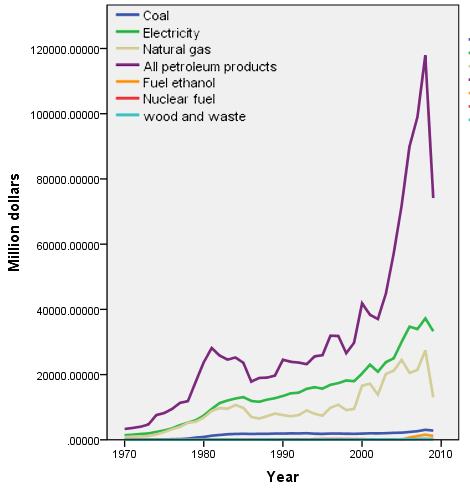
\includegraphics[width=3in]{TXTCV.png}
\caption{TXTCV} \label{fig:TXTCV}
\end{minipage}
\end{figure}



\section{Sub-Model.\Rmnum{1}:3E Evaluation Model}
\subsection{Result and Analysis}
To describe the energy situation of the four states, first, we need to define an indicator that describes the overall condition of energy.Energy is closely related to the economy and the environment. therefore, the impact of economic and environment can not be ignored as we consider the condition of energy.

So we study the paper \cite{zhaotao2008energy} and take it into consideration. For energy, we use total energy consumption and clean energy consumption as a proportion of total energy consumption; For economy, we use the GDP of each state and real GDP per capita of each state; For the environment, we use carbon dioxide emissions and temperature data. Finally, these data are integrated to represent our indicators of clean energy.
For the weight of the two kinds of data in all aspects, we use the method of principal component analysis and analytic hierarchy process to determine synthetically. This process can not only express the subjective will of policy makers, but also avoid the deviation of subjective wishes and the actual situation. In addtion, the original data can be fully utilized.Based on experience, we assume that subjective weights and objective weights are equally important, then the weight of each  indicator is
\begin{equation}
  W_{ti} = 0.5 W_{si} + 0.5 W_{oi} 
\end{equation}

First, we standardize on the six kinds of data. The way We use to standardize is the range-method . Formulas are as follows:\\

For positive indicators,

\begin{equation}
  Y_i = \frac{X_i - X_{min}}{X_{max} - X_{min}}
\end{equation}

For negative indicators,
\begin{equation}
  Y_i = \frac{X_{max} - X_i}{X_{max} - X_{min}}
\end{equation}

Therefore, the final calculation formula of energy, economy and environment is 
\begin{equation}
  E = \sum_{i=1}^{n} W_{ti} Y_{i} 
\end{equation}

We assume that energy, economy and environment are equally important to our indicators, so the formula is
\begin{equation}
  E^{*} = \frac{E_e + E_c + E_v}{3}
\end{equation}

The larger this indicator, the better the clean energy condition. Among them, as the reason of that carbon dioxide emissions is positive, the actual calculation need to take the opposite treatment.

After then, we make a statistical analysis of the energy status indicators of each state from 1980 to 2009, and make the figure of comprehensive energy status indicator time series in different states, as shown below.
\begin{figure}[htb]
  \centering
  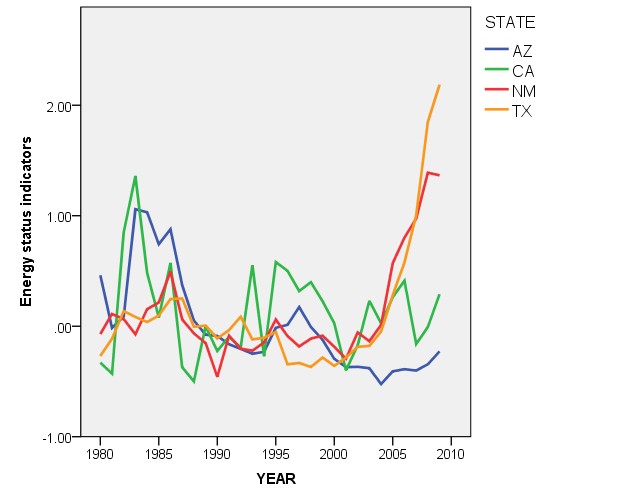
\includegraphics[width=12cm]{b1.png}
  \caption{Comprehensive energy status indicator time series} \label{fig: Comprehensive energy status indicator time series}
\end{figure}

As we can see, the beginning of the rapid economic growth leads to the indicator increasing. However, due to the impact of carbon dioxide emissions on  environmental factors, the indicators of all states began to decrease around 1987. Then, with the concept of sustainable development strengthened, each state proposed its own new energy policy and the indicator began to increase. As we can see in Texas and New Mexico, because of their energetic efforts to develop new energy sources, their indicators were increasing at a relatively faster rate.

Moreover, since there is a large amount of data in each state that affects the similarities and differences between the states, we analyze the renewable energy condition in each of the four states by making time series diagram of different states.

We plot the development trends of various renewable energy categories in Arizona over the past 50 years in figure.\ref{fig: Arizona renewable energy time series}.
\begin{figure}[htb]
  \centering
  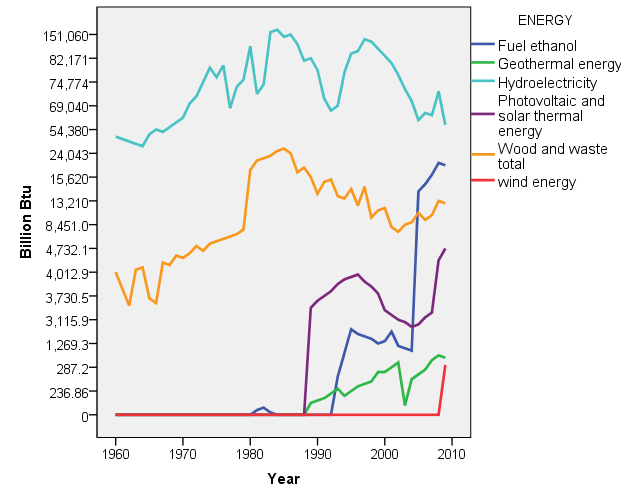
\includegraphics[width=12cm]{azre.png}
  \caption{Arizona renewable energy time series} \label{fig: Arizona renewable energy time series}
\end{figure}

As we can see, hydropower in Arizona is growing earlier and occupies a significant proportion of all renewable energy sources, followed by wood and waste products. Other renewable energy sources began to develop in the 1980s and 1990s. It is is notable that fuel ethanol and solar power are developing rapidly. By 2009, fuel ethanol consumption exceeded that of wood and waste, making it the second largest consumption of renewable energy.

An analysis of Arizona's geography and climate shows that Arizona has abundant solar energy resources, averaging 300 sunny days a year. However, due to the long-term high cost of photovoltaic energy, the growth rate has gradually slowed down after the initial rapid growth. The current cost of photovoltaic energy is estimated at 0.15-0.25 dollars / kWh, so the development is not satisfactory.\cite{AZretime}
Although the wind energy in Arizona is developing slowly, its development prospects are good. Located near the eastern edge of Mogollon Rim, eastern Arizona and eastern Arizona are geographically superior and resource-rich. There are also good wind resources on the edges and ridges across the state.\cite{AZwind}

We plot the development trends of various renewable energy categories in California over the past 50 years in figure.\ref{California renewable energy time series}.
\begin{figure}[htb]
  \centering
  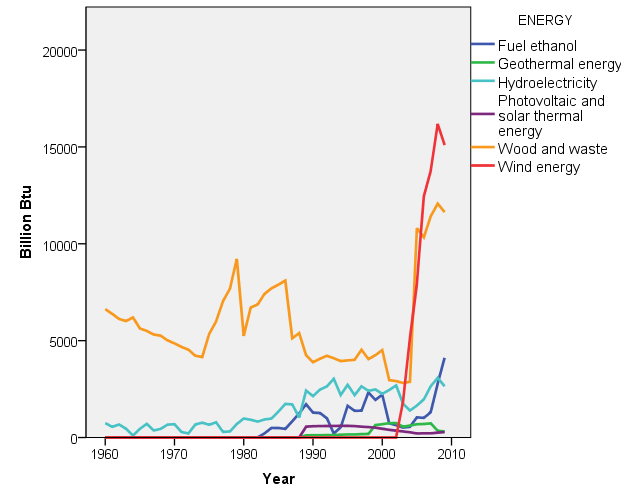
\includegraphics[width=12cm]{nmre.png}
  \caption{California renewable energy time series} \label{fig: California renewable energy time series}
\end{figure}

The figure shows that California's total renewable energy consumption is huge. All types of renewable energy consumption is similar to that in Arizona, where hydropower accounts for the highest share of all renewable energy sources, followed by wood and waste. Other renewable energy sources began to develop in the 1980s and 1990s. It is is notable that fuel ethanol is developing fastest. Unlike other sources of energy, California's geothermal energy has grown earlier and is consumed much more.

After analyzing the state of California, we can see it clear that the eastern part of California, especially the southern tip and the northeast end is a desert, so there may be more geothermal energy. In addition, due to the large population, there are also many energy consumption.

We plot the development trends of various renewable energy categories in New Mexico over the past 50 years in figure.\ref{fig: New Mexico renewable energy time series}.
\begin{figure}[htb]
  \centering
  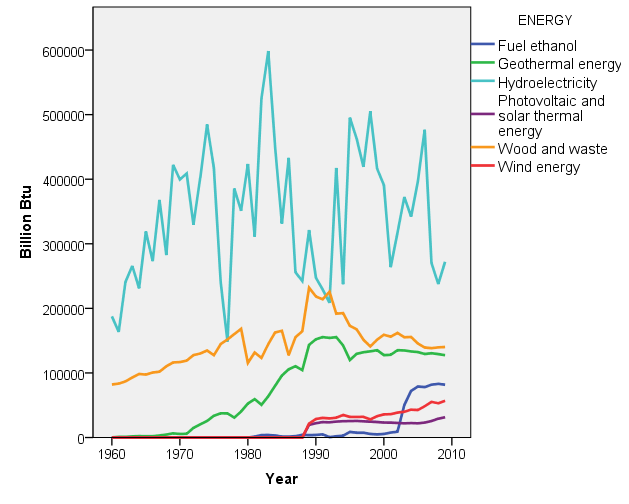
\includegraphics[width=12cm]{care.png}
  \caption{New Mexico renewable energy time series} \label{fig: New Mexico renewable energy time series}
\end{figure}

As we can see, the state's total renewable energy consumption is less. By 2005, the largest share of renewable energy was wood and waste. Wind energy has grown rapidly since 2005, making it the biggest consumption of renewable energy.

We plot the development trends of various renewable energy categories in Texas over the past 50 years in figure.\ref{fig: Texas renewable energy time series}.
\begin{figure}[htb]
  \centering
  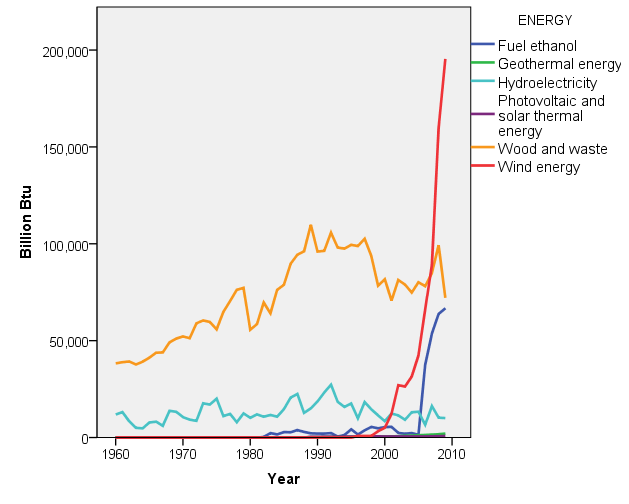
\includegraphics[width=12cm]{txre.png}
  \caption{Texas renewable energy time series} \label{fig: Texas renewable energy time series}
\end{figure}

It can be seen that Texas is very much like New Mexico in the use of wind energy and wood and waste.After analysis of Texas data, we find that at present Texas is the largest state in the United States with the highest wind energy generation. What supers us is taht the wind energy consumptiion has been increased so fast in past ten years. The paper \cite{Langniss2003The} shows that the reason is the state's renewables portfolio standard (RPS), which forces RPS Power suppliers proactively use large-scale wind and other renewable energy to generate electricity.

\subsection{Conclution}
A comparison of all the figures above demonstrates that Arizona and California are similar, while new Mexico and Texas are similar. Renewable energy sources in Arizona and California account for a large proportion of renewable energy. Wind energy in New Mexico and Texas accounts for a large proportion of renewable energy. As the result of the difference between different states in geography and climate, Arizona mainly develops solar energy while California, imainly developing geothermal energy,  New Mexico and Texas mainly developing wind energy.In addition, each state's fuel ethanol energy has a certain development.

\section{Determing ``best'' profile}
In order to facilitate the further processing of the following problems, we use gray relational analysis.
\subsection{gray relational analysis}
Gray system theory puts forward the concept of analyzing the gray relational degree of each subsystem. It intends to seek the numerical relationship among the subsystems (or factors) in the system through certain methods.
Therefore, gray relational analysis provides a quantitative measure of a system development trend and is very suitable for dynamic history analysis.\cite{AZretime}

\subsection{Calculation Step}
First, Identify reference sequences that reflect system behavior characteristics and comparison sequences that affect system behavior.
The sequence of data that reflects the behavior of the system is called the reference sequence. Factors affecting the behavior of the system composed of data series, is called the comparison sequence.

After obtaining the reference sequence and the comparison sequence, the reference sequence and the comparison sequences should be treated dimensionless.
Due to the different physical meaning of each factor in the system, the dimensionality of the data is not necessarily the same, which is not convenient for comparison, or it is difficult to get the correct conclusion in comparison. Therefore, in the analysis of grey relational degree, it is generally necessary to conduct dimensionless data processing.
\newline
Select reference sequence,
\begin{equation}
  x_0 = \{x_0(k) | k=1,2,\cdots,n \} = (x_0(1), x_0(2), \cdots, x_0(n))
\end{equation}
Suppose there are m number of comparisons,
\begin{equation}
x_i = \{x_i(k) | k=1,2,\cdots,n\} = (x_i(1), x_i(2), \cdots, x_i(n)), i = 1,2,\cdots,m 
\end{equation}
Where k represents the moment, a total of n moments.

Before calculating the correlation coefficient, the comparison sequence need to be treated dimensionless. The common dimensionless methods are average method and initialization method.
What we use is the initialization method.
Here $ x_i '(k) $ indicates the comparison sequence just screened. $ x_i (k) $ is the new processed comparison sequence.

After that, the gray correlation coefficient $r_i(k)$ between the reference sequence and the comparison sequence can be calculated.
The so-called correlation coefficient, is substantially between degree of difference curve geometry. Therefore, the size of the difference between the curves can be used as a measure of the degree of association
For a reference sequence $ x_0 $, there are several comparison sequences $ x_1, x_2, \ cdots, x_m $. The correlation coefficient $ r_i (k) $ of each comparison sequence and the reference sequence at each moment (ie, points in the curve) can be calculated by following formula: Where $\rho$ is the resolution coefficient, generally between 0 to 1, usually take 0.5.
\begin{equation}
  r_i(k) = \frac{\min\limits_{i} \min\limits_{k}| x_0(k) - x_i(k)| + \rho \times \min\limits_{i} \min\limits_{k}| x_0(k) - x_i(k)|}{|x_0(k) - x_i(k)| + \rho \times \min\limits_{i} \min\limits_{k}| x_0(k) - x_i(k)|},\quad k=1,2,\cdots,n
\end{equation}

\newpage
\setcounter{page}{2}
\pagestyle{fancy} 
\rhead{\small\sffamily  \rmnum{\thepage}}

\bibliographystyle{siam}
\bibliography{ref}


\begin{appendices}


\begin{minipage}{\textwidth}
  \begin{minipage}[t]{0.45\textwidth}
    \centering
      \makeatletter\def\@captype{table}\makeatother\caption{txCO2}
      \begin{tabular}{|l|c|}
        \hline
        date & million metric tons of CO2 \\ \hline
        1980 & 496.5                      \\ \hline
        1981 & 483.4                      \\ \hline
        1982 & 461.1                      \\ \hline
        1983 & 467.1                      \\ \hline
        1984 & 492.7                      \\ \hline
        1985 & 498.7                      \\ \hline
        1986 & 496.2                      \\ \hline
        1987 & 502.1                      \\ \hline
        1988 & 534.9                      \\ \hline
        1989 & 554.9                      \\ \hline
        1990 & 565.1                      \\ \hline
        1991 & 560.2                      \\ \hline
        1992 & 559.9                      \\ \hline
        1993 & 577.8                      \\ \hline
        1994 & 576.9                      \\ \hline
        1995 & 581.5                      \\ \hline
        1996 & 624.9                      \\ \hline
        1997 & 651.4                      \\ \hline
        1998 & 656.6                      \\ \hline
        1999 & 633.3                      \\ \hline
        2000 & 657.6                      \\ \hline
        2001 & 651.5                      \\ \hline
        2002 & 661.6                      \\ \hline
        2003 & 655.5                      \\ \hline
        2004 & 649.6                      \\ \hline
        2005 & 612.2                      \\ \hline
        2006 & 623.4                      \\ \hline
        2007 & 620                        \\ \hline
        2008 & 585                        \\ \hline
        2009 & 550.1                      \\ \hline
        2010 & 582.5                      \\ \hline
        2011 & 601.5                      \\ \hline
        2012 & 596.3                      \\ \hline
        2013 & 623                        \\ \hline
        2014 & 625.3                      \\ \hline
        2015 & 625.8                      \\ \hline
        \end{tabular}
    \end{minipage}
    \begin{minipage}[t]{0.45\textwidth}
    \centering
          \makeatletter\def\@captype{table}\makeatother\caption{nmCO2}
          \begin{tabular}{|l|c|}
            \hline
            date & million metric tons of CO2 \\ \hline
            1980 & 44.9                       \\ \hline
            1981 & 44                         \\ \hline
            1982 & 45.1                       \\ \hline
            1983 & 48.6                       \\ \hline
            1984 & 46.2                       \\ \hline
            1985 & 46.5                       \\ \hline
            1986 & 43                         \\ \hline
            1987 & 46.2                       \\ \hline
            1988 & 47.9                       \\ \hline
            1989 & 50.4                       \\ \hline
            1990 & 53.3                       \\ \hline
            1991 & 49.2                       \\ \hline
            1992 & 51.7                       \\ \hline
            1993 & 52.6                       \\ \hline
            1994 & 52.5                       \\ \hline
            1995 & 51.1                       \\ \hline
            1996 & 52.6                       \\ \hline
            1997 & 56                         \\ \hline
            1998 & 55.5                       \\ \hline
            1999 & 56.4                       \\ \hline
            2000 & 58.2                       \\ \hline
            2001 & 58.3                       \\ \hline
            2002 & 55.3                       \\ \hline
            2003 & 57.6                       \\ \hline
            2004 & 58.7                       \\ \hline
            2005 & 59.3                       \\ \hline
            2006 & 59.8                       \\ \hline
            2007 & 59                         \\ \hline
            2008 & 56.4                       \\ \hline
            2009 & 57.3                       \\ \hline
            2010 & 53.3                       \\ \hline
            2011 & 55.7                       \\ \hline
            2012 & 53.6                       \\ \hline
            2013 & 53.2                       \\ \hline
            2014 & 50.1                       \\ \hline
            2015 & 50.2                       \\ \hline
            \end{tabular}
  \end{minipage}
\end{minipage}

\begin{minipage}{\textwidth}
  \begin{minipage}[t]{0.45\textwidth}
   \centering
      \makeatletter\def\@captype{table}\makeatother\caption{caCO2}
      \begin{tabular}{|l|c|}
        \hline
        date & million metric tons of CO2 \\ \hline
        1980 & 348.4                      \\ \hline
        1981 & 337                        \\ \hline
        1982 & 299.9                      \\ \hline
        1983 & 293                        \\ \hline
        1984 & 319.5                      \\ \hline
        1985 & 324.2                      \\ \hline
        1986 & 309.5                      \\ \hline
        1987 & 340.1                      \\ \hline
        1988 & 348.2                      \\ \hline
        1989 & 363.5                      \\ \hline
        1990 & 363.9                      \\ \hline
        1991 & 351.7                      \\ \hline
        1992 & 356.1                      \\ \hline
        1993 & 345.5                      \\ \hline
        1994 & 362.4                      \\ \hline
        1995 & 351.4                      \\ \hline
        1996 & 350.5                      \\ \hline
        1997 & 353                        \\ \hline
        1998 & 363.4                      \\ \hline
        1999 & 367                        \\ \hline
        2000 & 382.4                      \\ \hline
        2001 & 386.9                      \\ \hline
        2002 & 386.1                      \\ \hline
        2003 & 373.8                      \\ \hline
        2004 & 392.3                      \\ \hline
        2005 & 389.3                      \\ \hline
        2006 & 397.5                      \\ \hline
        2007 & 402.5                      \\ \hline
        2008 & 385.7                      \\ \hline
        2009 & 372                        \\ \hline
        2010 & 365.9                      \\ \hline
        2011 & 352.2                      \\ \hline
        2012 & 357.1                      \\ \hline
        2013 & 359.8                      \\ \hline
        2014 & 356.7                      \\ \hline
        2015 & 363.5                      \\ \hline
        \end{tabular}
   \end{minipage}
   \begin{minipage}[t]{0.45\textwidth}
    \centering
         \makeatletter\def\@captype{table}\makeatother\caption{azCO2}
         \begin{tabular}{|l|c|}
          \hline
          date & million metric tons of CO2 \\ \hline
          1980 & 52.7                       \\ \hline
          1981 & 59.6                       \\ \hline
          1982 & 58.2                       \\ \hline
          1983 & 53.9                       \\ \hline
          1984 & 58.2                       \\ \hline
          1985 & 60.7                       \\ \hline
          1986 & 55.9                       \\ \hline
          1987 & 56.1                       \\ \hline
          1988 & 59.3                       \\ \hline
          1989 & 65.2                       \\ \hline
          1990 & 62.8                       \\ \hline
          1991 & 63.7                       \\ \hline
          1992 & 66.5                       \\ \hline
          1993 & 69                         \\ \hline
          1994 & 71.7                       \\ \hline
          1995 & 66.7                       \\ \hline
          1996 & 68.4                       \\ \hline
          1997 & 71.6                       \\ \hline
          1998 & 76.5                       \\ \hline
          1999 & 80.4                       \\ \hline
          2000 & 86.1                       \\ \hline
          2001 & 88.4                       \\ \hline
          2002 & 87.8                       \\ \hline
          2003 & 89.6                       \\ \hline
          2004 & 96.6                       \\ \hline
          2005 & 96.7                       \\ \hline
          2006 & 99.9                       \\ \hline
          2007 & 101.9                      \\ \hline
          2008 & 102.3                      \\ \hline
          2009 & 93.4                       \\ \hline
          2010 & 95.2                       \\ \hline
          2011 & 93.3                       \\ \hline
          2012 & 91.3                       \\ \hline
          2013 & 95.1                       \\ \hline
          2014 & 93.1                       \\ \hline
          2015 & 90.9                       \\ \hline
          \end{tabular}
    \end{minipage}
 \end{minipage}




\begin{proof}   %插入证明
  x
\end{proof}

\newtheorem{lemma}{Lemma}%只需在第一个引理开始之前出现一次  
\begin{lemma}  
If $f\in C_{L}^{1,1}(\mathbb{R}^{n})$, then $\forall \textbf{x},\textbf{y}\in\mathbb{R}^{n}$ we have  
\begin{equation}  
\left|{f(\textbf{y})-f(\textbf{x})-\nabla f(\textbf{x})^{T}(\textbf{y}-\textbf{x})}\right|\le\frac{L}{2}\left\|{\textbf{y}-\textbf{x}}\right\|^{2}.  
%\label{eq:eq5}  
\end{equation}  
%\label{lem:lem1}  
\end{lemma} 
\section{First appendix}

\lipsum[13]

% 代码插入
Here are simulation programmes we used in our model as follow.\\

\textbf{\textcolor[rgb]{0.98,0.00,0.00}{Input matlab source:}}
\lstinputlisting[language=Matlab]{./code/mcmthesis-matlab1.m}

\section{Second appendix}

some more text \textcolor[rgb]{0.98,0.00,0.00}{\textbf{Input C++ source:}}
\lstinputlisting[language=C++]{./code/mcmthesis-sudoku.cpp}

\end{appendices}
\end{document}

